\section{Fallbeispiele}

%%% Folie
{
\scriptsize

\begin{frame}[allowframebreaks]{Entwurf eines mobilen Datenloggers}
    \begin{block}{Problemstellung}
        \Justified{
            \smallskip
            Der internationale Versand hochwertiger Güter birgt viele Gefahren.
            Raue Umweltbedingungen, falsche Lagerung und unsachgemäße Behandlung
            können schnell zu Beschädigungen führen, deren Zeitpunkt und Ursache
            nachträglich nur schwer nachgewiesen werden kann. Es soll daher ein
            mobiler Datenlogger entworfen werden, der die Waren auf ihrer Reise
            begleitet und kontinuierlich verschiedene Umweltparameter aufzeichnet.
            Die gesammelten Werte sollen auf einer SD-Karte gespeichert und am
            Ende der Reise an einen Server im Internet übertragen werden.
        }
    \end{block}

    \begin{block}{Hardware}
        \smallskip
        Folgende Single Board Computer stehen zur Auswahl:
        \smallskip

        \begin{columns}
            \column[b]{0.2\textwidth}
            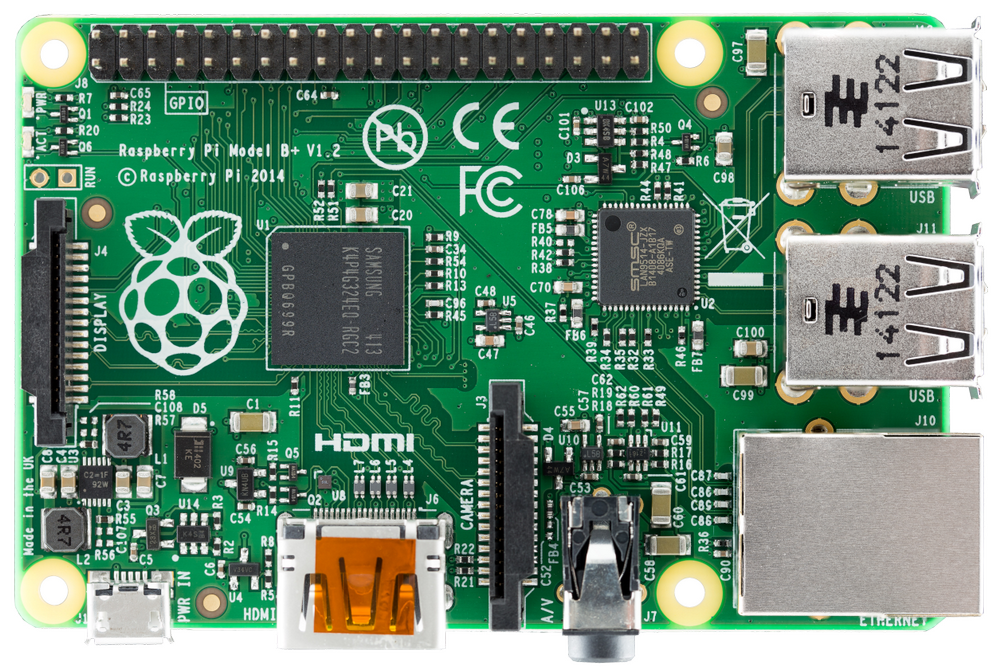
\includegraphics[width=\textwidth]{99-beispiele/img/raspberrypi}

            \column[b]{0.2\textwidth}
            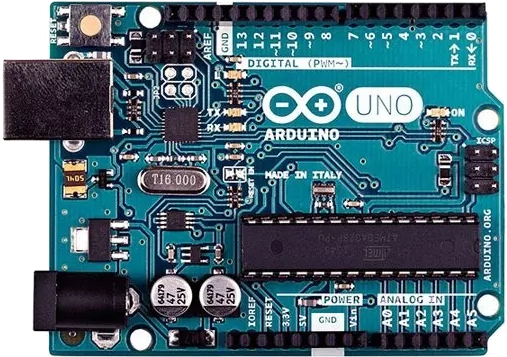
\includegraphics[width=\textwidth]{99-beispiele/img/arduino}

            \column[b]{0.2\textwidth}
            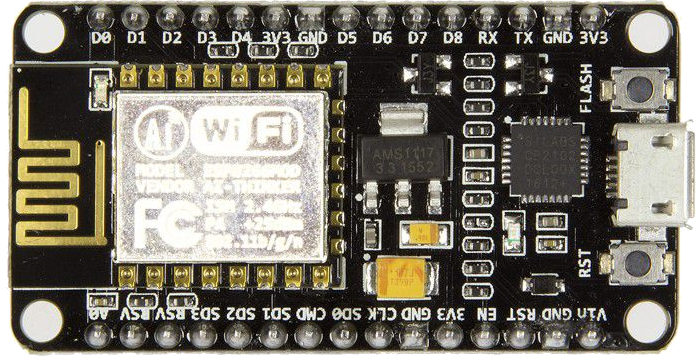
\includegraphics[width=\textwidth]{99-beispiele/img/esp8266}

            \column[b]{0.2\textwidth}
            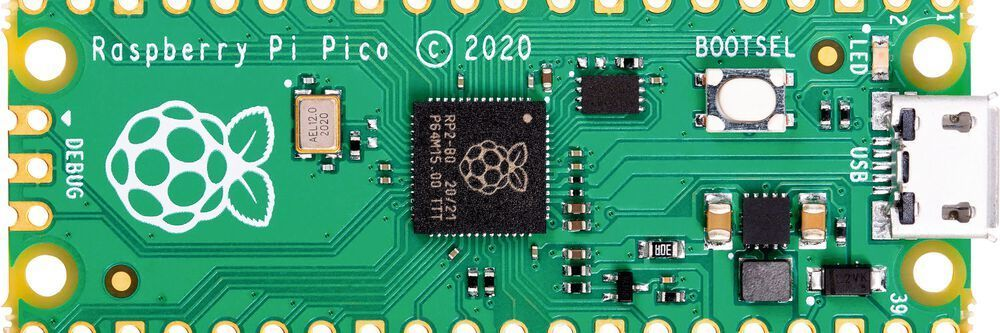
\includegraphics[width=\textwidth]{99-beispiele/img/pi-pico}
        \end{columns}
        \begin{columns}
            \column[b]{0.2\textwidth}
            \textsc{Raspberry Pi 4}

            \column[b]{0.2\textwidth}
            \textsc{Arduino Uno}

            \column[b]{0.2\textwidth}
            \textsc{ESP 8266}

            \column[b]{0.2\textwidth}
            \textsc{Raspberry Pi Pico}
        \end{columns}
    \end{block}

    \begin{block}{Sensoren}
        \smallskip
        Folgende Sensoren sollen verwendet werden:
        \medskip

        \begin{columns}
            \column{0.33\textwidth}
            \textbf{KY-002}: Erschütterungsschalter

            \column{0.33\textwidth}
            \textbf{KY-015}: DHT11-Kombisensor

            \column{0.33\textwidth}
            \textbf{KY-017}: Neigungsschalter
        \end{columns}
        \smallskip
        \begin{columns}
            \column{0.33\textwidth}
            \textbf{KY-031}: Klopfsensor

            \column{0.33\textwidth}
            \textbf{KY-024}: Magnetfeldsensor

            \column{0.33\textwidth}
        \end{columns}
    \end{block}

    \framebreak

    \begin{block}{Weitere Hardware}
        \Justified{
            \smallskip
            Die Internetverbindung soll über WLAN hergestellt werden. Um die Verbindungsdaten
            nicht fest in die Firmware einprogrammieren zu müssen, und um einen Namen für jede
            Sendung eingeben zu können, sollen darüber hinaus ein LCD-Display ein paar Buttons
            zur Dateneingabe angeschlossen werden.
        }

        \Justified{
            \medskip
            LCD-Display und WLAN soll im laufenden Betrieb ausgeschaltet sein, um
            Strom zu sparen. Eine blinkende LED soll stattdessen signalisieren,
            dass die Aufzeichnung läuft.
        }
    \end{block}

    \begin{block}{Zu beantwortende Fragen}
        \begin{itemize}
            \item Was sind die Vor- oder Nachteile des jeweiligen Single Board Computers?
            \item Wie groß muss die Stromversorgung jeweils dimensioniert werden?
            \item Welche Zusatzhardware wird für die WLAN-Verbindung benötigt?
            \item Welche Zusatzhardware wird für den SD-Kartenslot benötigt?
            \item Wie müssen die Sensoren mit dem Embedded Board verbunden werden?
            \item Welche Möglichkeiten gibt es, ein LCD-Display anzubinden?
            \item Wie kann die Dateneingabe für den Namen der Sendung etc. realisiert werden?
        \end{itemize}

        \bigskip
        Erstellen Sie eine Folienpräsentation und stellen Sie diese am Ende der Vorlesung vor.
    \end{block}
\end{frame}
}
